\chapter{Type II Prediction: System Identification}\label{ch:predictor_t2}

\section{Premise}

\begin{quote}
\noindent
The state of a structure as it experiences an event is assumed to be characterized by its displacement $\displ$ and velocity $\veloc$. It is governed by Newton's laws of motion (same as \cref{eq:newton-discrete} but repeated here for convenience):
\begin{equation*}
    \Mass \accel = \extern -  \intern(\displ,\veloc), %\force (\displ, \veloc, \accel) = \mathbf{f}
\end{equation*}
where $\accel$ is the acceleration associated with the state of the structure, $\intern$ characterizes the internal resisting force produced by the structure in response to its configuration, and $\extern$ is the external loading that is imposed by the event. \glspl{predictor-t2} are premised on the idea that if general constraints on $\Mass$ and $\intern$ are \emph{assumed} and $\extern$ and $\accel$ are \emph{given}, then the function $\intern$ can be approximately \emph{determined} by algebra.
%
On the \gls{platform}, this is realized by prescribing the domain and range of $\intern$ and then using \emph{system identification} methods to fit $\intern$ to directly observed loading and acceleration data.
\end{quote}


\section{Modeling}
\label{sec:modeling_predictor_II}
\cref{tab:sysid_methods} presents the methods available to use as system identification predictors. There are two main categories of methods: state-space models and input/output models. State-space models (see \cref{sec:mdof_theory}) use matrix methods to estimate a set of differential equations relating input, state, and output. Often, a stabilization diagram (\cref{fig:stabilization}) is used to interpret the results of state-space models. Identified periods and damping ratios are those that are consistent across model orders. Input/output models (see \cref{sec:fourier}), such as transfer functions, use complex analysis to estimate a direct relationship between the input and output. Often, a frequency response function (\cref{fig:transfer_plot}) is used to interpret the results of input/output models. Identified periods are those that are associated with peaks in the amplitude of the transfer function.
\begin{table}[h!]
    \centering
    \begin{tabular}{lll}
\toprule
        \textbf{Name} & \textbf{Abbreviation} & \textbf{Classification} \\ \hline
        Observer Kalman ID-Eigensystem Realization Algorithm & OKID-ERA & State-Space \\
        System Realization using Information Matrix & SRIM & State-Space \\
        Response Spectrum Transfer Function & RSTF & Input/Output\\
        Fourier amplitude Spectrum Transfer Function & FSTF & Input/Output\\
        Power Spectrum Transfer Function & PSTF & Input/Output\\
\bottomrule
    \end{tabular}
    \caption{Methods of system IDentification (ID).}
    \label{tab:sysid_methods}
\end{table}
\begin{figure}[h!]
    \centering
    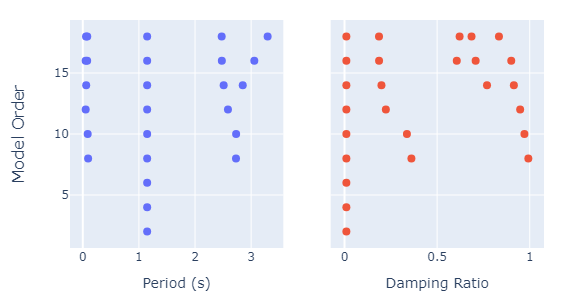
\includegraphics[width=0.7\linewidth]{Part II/figures/predictors/stabilization.png}
    \caption{Stabilization diagram, commonly used to interpret state-space model results.}
    \label{fig:stabilization}
\end{figure}
\begin{figure}[h!]
    \centering
    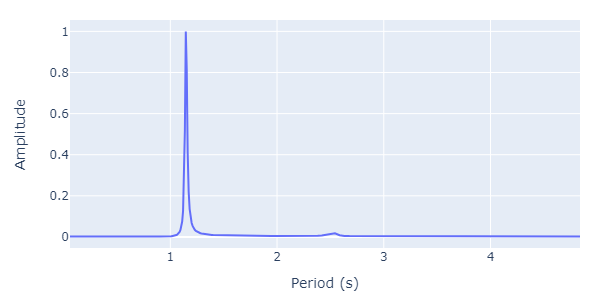
\includegraphics[width=0.7\linewidth]{Part II/figures/predictors/transfer_plot.png}
    \caption{Frequency response function, commonly used to interpret input/output model results.}
    \label{fig:transfer_plot}
\end{figure}

Generally, state-space models are more suitable for systems with multiple inputs and outputs, while input/output models are more suitable for single-input, single-output systems. Out of the state-space models, SRIM is generally preferable when little to no correlation between future inputs and the current state is expected. OKID-ERA is generally preferable when it is expected that the system's impulse response can be estimated from the forced response. Although all input/output models give similar results, the response spectrum transfer function is the most familiar to practicing engineers.

% \begin{table}[]
%     \centering
%     \begin{tabular}{ll}        
%     \textbf{Name} & \textbf{Abbreviation} \\ \hline
%         Response Spectrum Transfer Function & RSTF \\
%         Fourier Amplitude Spectrum Transfer Function & FSTF \\
%         Power Spectrum Transfer Function & PSTF \\
%         % Frequency Domain Decomposition & FDD \\
%     \end{tabular}
%     \caption{Methods: Input/Output System Identification Models}
%     \label{tab:input_output_methods}
% \end{table}

\subsection{Configuration Interface}

The following notes and figures describe the workflow for interested users to build a system identification predictor on the \BRACE{} platform.

\begin{itemize}
    \item From an asset's Structure Profile, select the Configure Predictors button (\tikz\node[squarednode,fill=cyan,scale=0.7] {\small 1};, \cref{fig:struct_profile}).
    \item Select, New System ID (\tikz\node[squarednode,fill=cyan,scale=0.7] {\small 2};, \cref{fig:predictors_page}).
    \item Complete the Predictor Builder form to configure a system identification predictor (\cref{fig:config_form}): \begin{itemize}
        \item Provide a name for the predictor (\tikz\node[circle,fill=cyan,scale=0.6] {\small 3};).
        \item Select Method (methods are discussed broadly in \cref{sec:describe_sysid_configs} and in depth in \cref{sec:mdof_theory}) (\tikz\node[circle,fill=cyan,scale=0.6] {\small 4};).
        \item Specify decimation (downsampling) factor (\tikz\node[circle,fill=cyan,scale=0.6] {\small 5};).
        \item Specify method-specific model parameters (\tikz\node[circle,fill=cyan,scale=0.6] {\small 6};).
        \item Select Channels. Define input and output signal identification numbers, as defined in the Structure Profile, e.g., \cref{fig:struct_profile}, (\tikz\node[squarednode,fill=cyan,scale=0.7] {\small 7};).
        \item Select Submit (\tikz\node[squarednode,fill=cyan,scale=0.7] {\small 8};).
    \end{itemize}
    \item Once the form is completed, the system identification predictor is populated on the Predictors page (\tikz\node[squarednode,fill=cyan,scale=0.7] {\small 9};, \cref{fig:predictors_page}).
\end{itemize}
\begin{figure}[h!]
\centering
  \begin{tikzpicture}
    \node [above right, inner sep=0] (image) at (0,0) {
        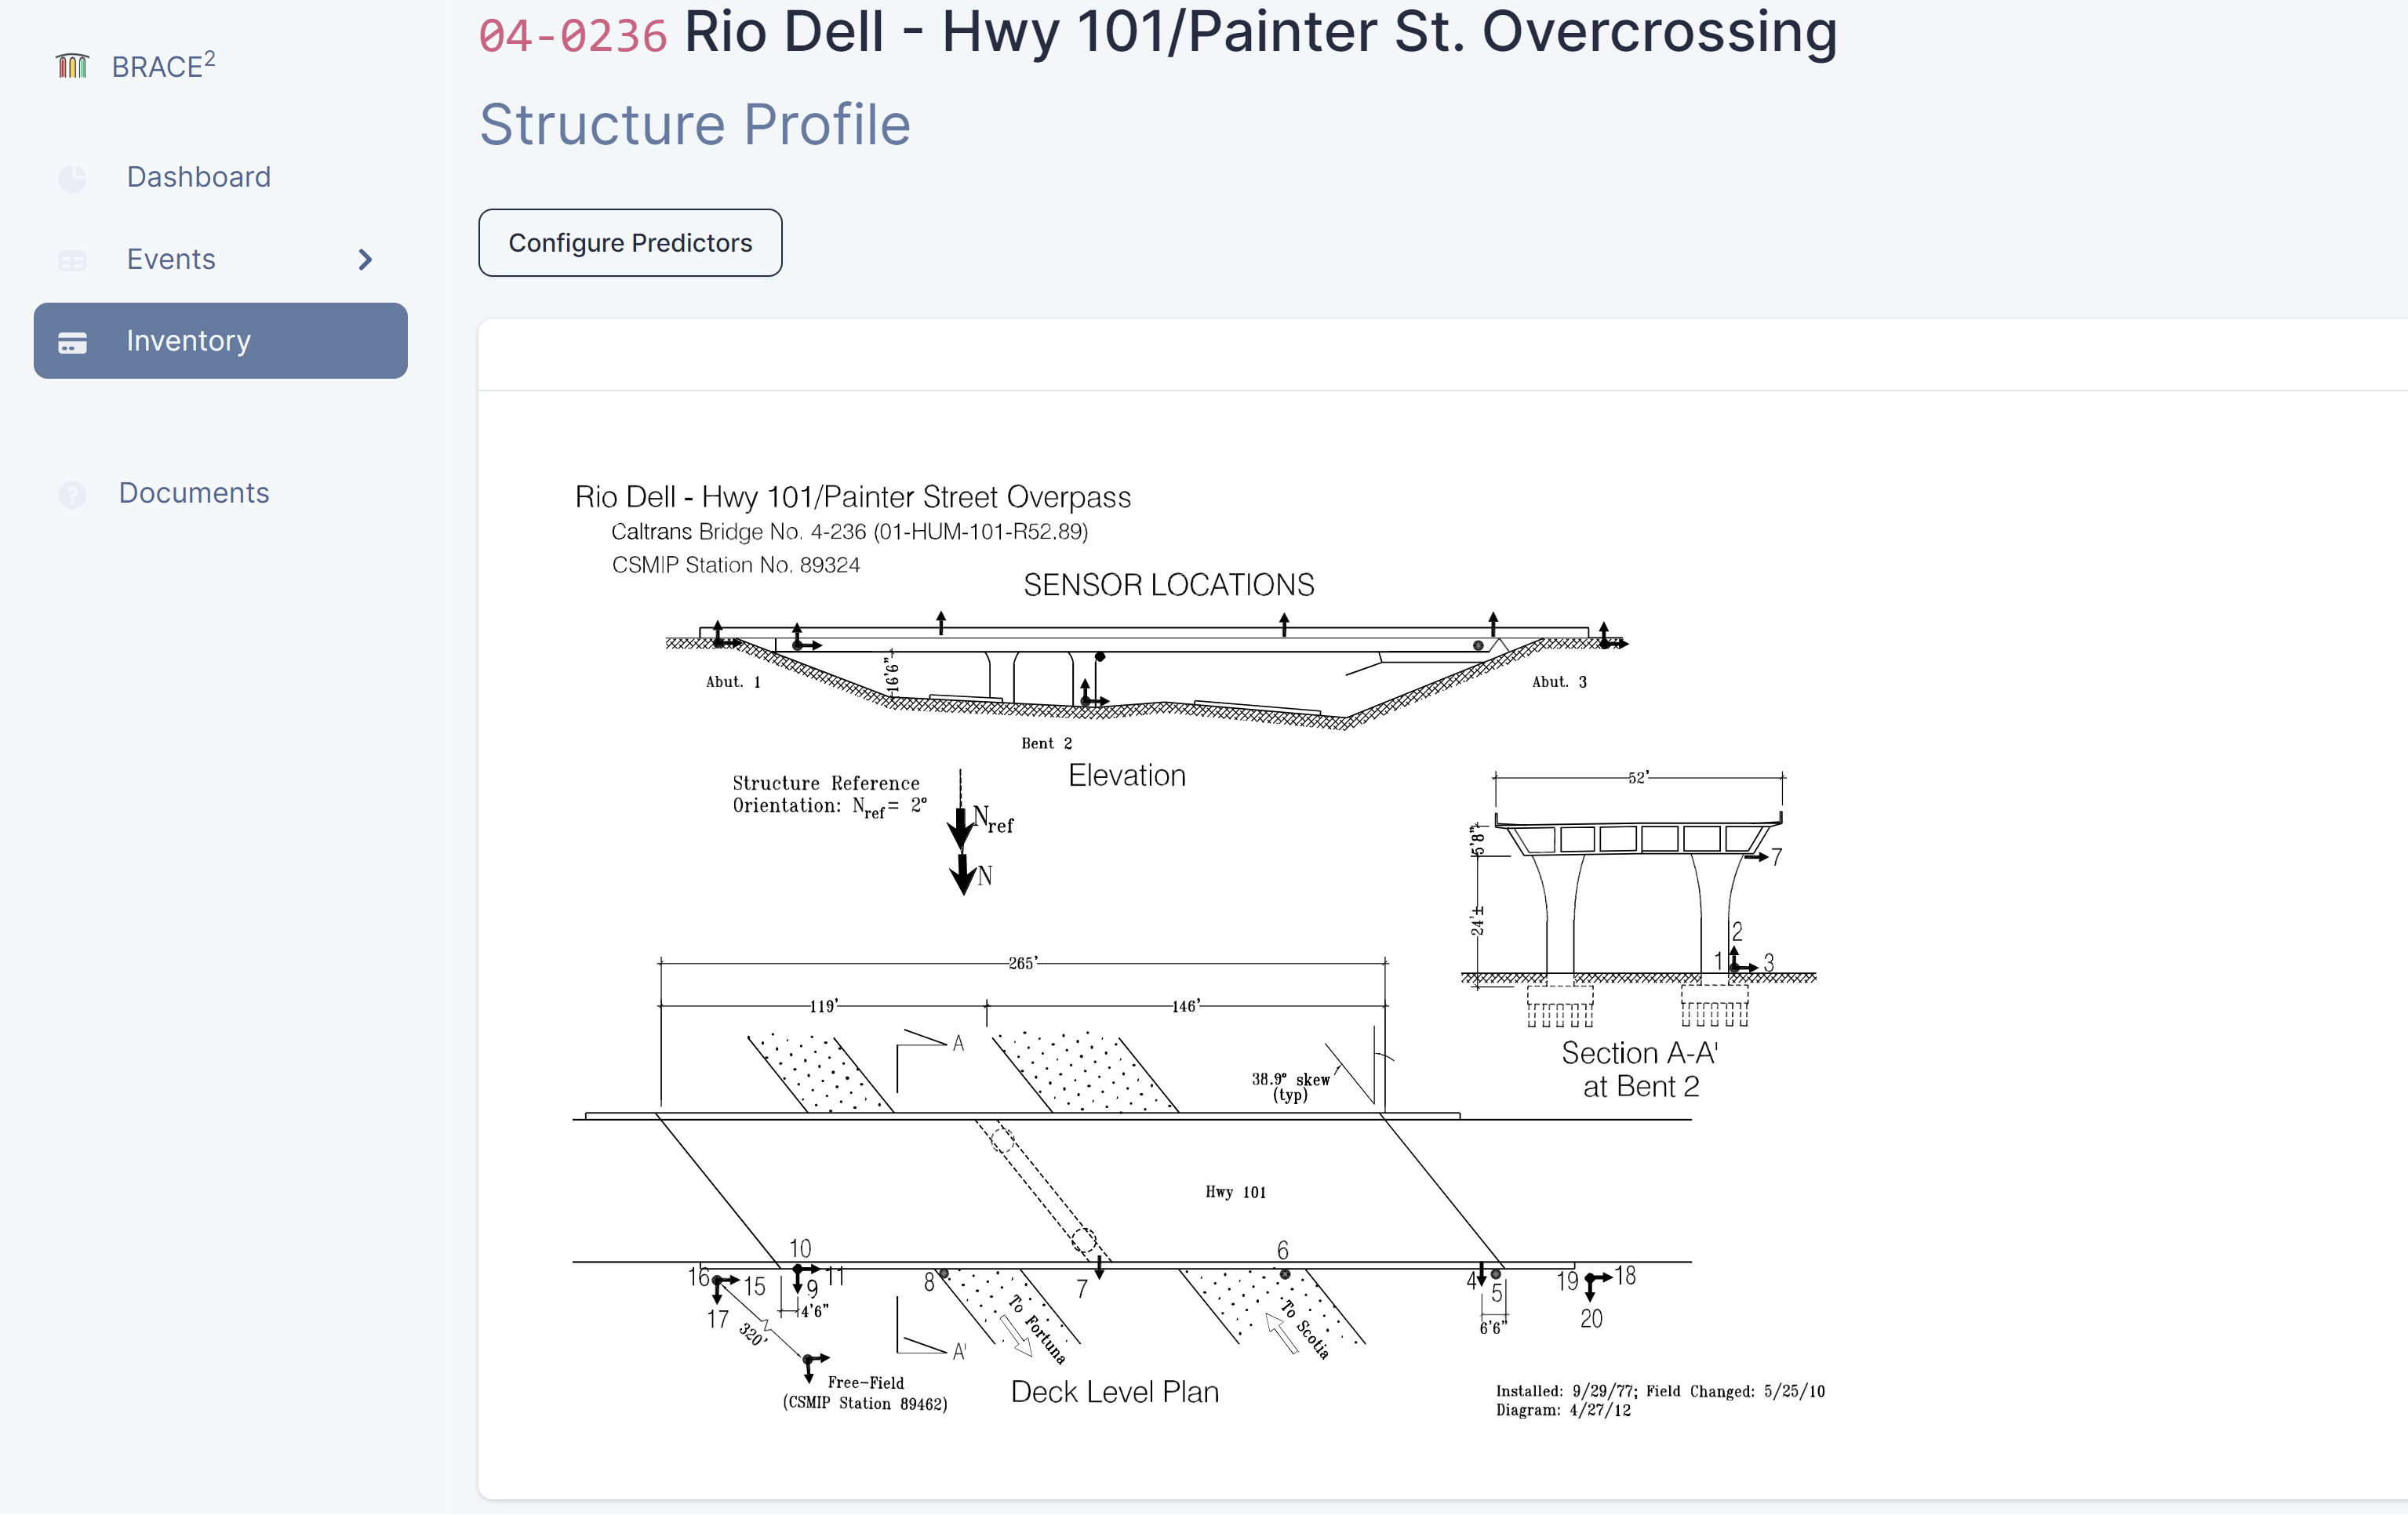
\includegraphics[width=\linewidth]{Part II/figures/predictors/config_button_3.png}
    };
    % Create scope with normalized axes
    \begin{scope}[
    x={($0.1*(image.south east)$)},
    y={($0.1*(image.north west)$)}]
% Annotations
    \draw[very thick,cyan] (2,8.1) rectangle (3.6,8.7) 
        node[below left,black,fill=cyan]{1};
  \end{scope}
  \end{tikzpicture}
\caption{An example asset's Structure Profile.}
\label{fig:struct_profile}
\end{figure}
\begin{figure}[h!]
\centering
  \begin{tikzpicture}
    \node [above right, inner sep=0] (image) at (0,0) {
        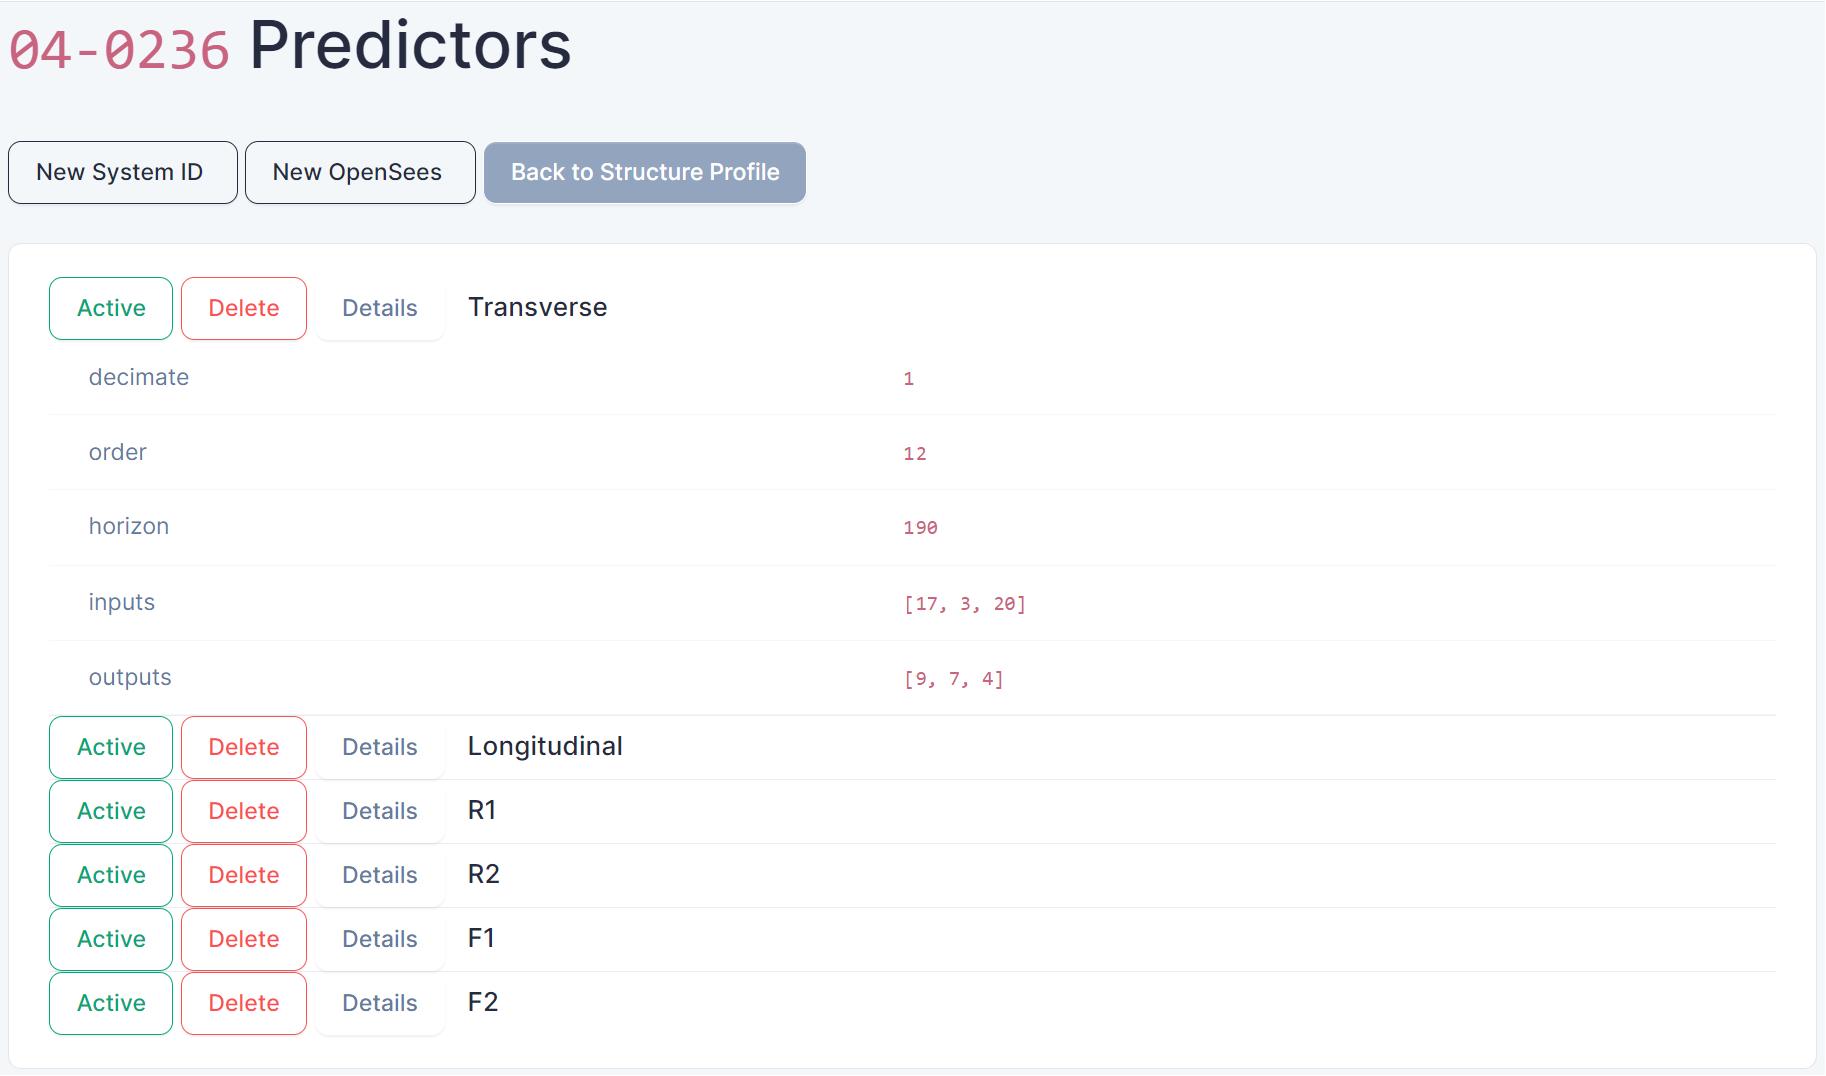
\includegraphics[width=\linewidth]{Part II/figures/predictors/predictors_2.png}
    };
    % Create scope with normalized axes
    \begin{scope}[
    x={($0.1*(image.south east)$)},
    y={($0.1*(image.north west)$)}]
% Annotations
    \draw[very thick,cyan] (0,8) rectangle (1.45,8.8) 
        node[below left,black,fill=cyan]{2};
    \draw[very thick,cyan] (0,3.4) rectangle (9.9,7.8) 
        node[below left,black,fill=cyan]{9};
  \end{scope}
  \end{tikzpicture}
\caption{An example asset's Predictors page.}
\label{fig:predictors_page}
\end{figure}
\begin{figure}[h!]
\centering
  \begin{tikzpicture}
    \node [above right, inner sep=0] (image) at (0,0) {
        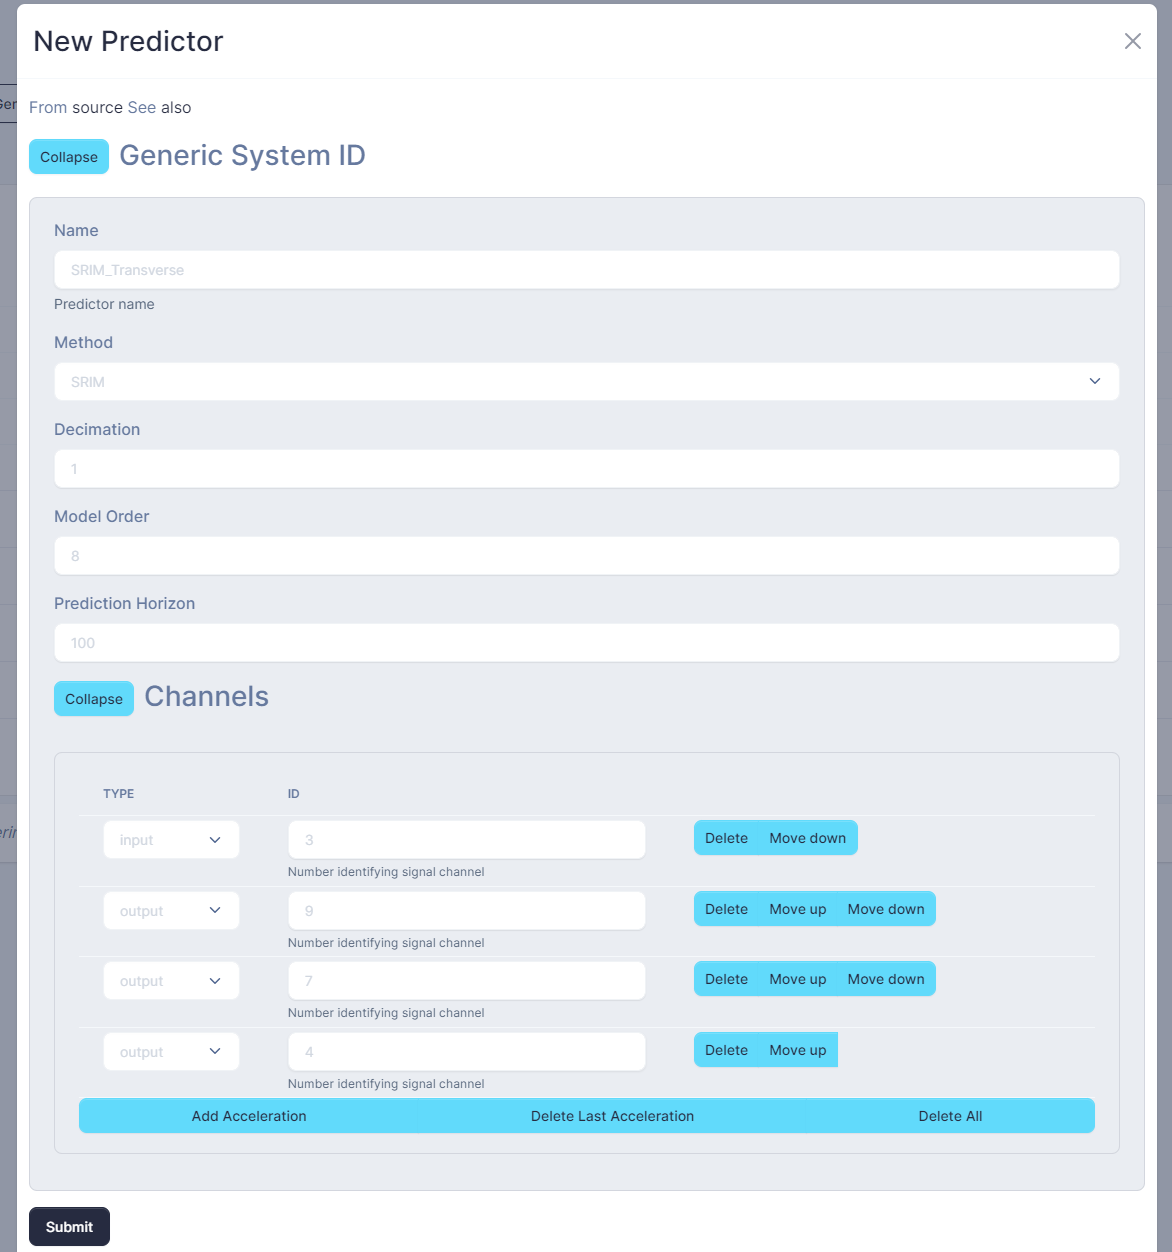
\includegraphics[width=\linewidth]{Part II/figures/predictors/config_form.png}
    };
    % Create scope with normalized axes
    \begin{scope}[
    x={($0.1*(image.south east)$)},
    y={($0.1*(image.north west)$)}]
% Annotations
    \node[circle,fill=cyan] at (3,7.9){\small 3};
    \node[circle,fill=cyan] at (3,7){\small 4};
    \node[circle,fill=cyan] at (3,6.3){\small 5};
    \node[circle,fill=cyan] at (3,5.6){\small 6};
    \node[circle,fill=cyan] at (3,4.9){\small 6};
    \draw[very thick,cyan] (0.5,0.8) rectangle (9.5,4) 
        node[below left,black,fill=cyan]{7};    
    \draw[very thick,cyan] (0.2,0.05) rectangle (1.4,0.4) 
        node[below left,black,fill=cyan]{8};
  \end{scope}
  \end{tikzpicture}
\caption{Predictor Builder form for configuring a generic system identification predictor.}
\label{fig:config_form}
\end{figure}

For the structure in \cref{fig:struct_profile}, an example system identification predictor is built in \cref{fig:config_form}. The method is SRIM with a decimation factor of 1, a model order of 8, a prediction horizon of 100, input channel 3 (aligned with the North-South axis and located at the base of the North column of the shown skewed bent), and output channels 9, 7, and 4 (in the transverse direction at the superstructure from East to middle to West).

\subsection{Configuration Options}\label{sec:describe_sysid_configs}

\cref{tab:sysid_options} presents the options available for each system identification predictor, including a top-level view of their interpretation. For most options, the default value provided by the configuration form is generally acceptable, but the input and output channels must be selected based on the sensor locations, identified by their identification number in the Structure Profile. In addition, adjustment of the model order should be considered. Model order is an option only applicable for state-space models. As the model order increases, the number of considered natural modes of vibration increases. Accordingly, model complexity and computational time can also increase. Therefore, it is recommended not to over-define the model by setting the model order too high. For example, for an ordinary standard reinforced concrete bridge with a two-span superstructure supported on a single column bent, a model order between $4$ and $20$ is generally acceptable and expected to capture the significantly contributing modes of the structural system (see \cref{sec:modal} for a discussion on optimal model order).
\begin{table}[h!]
    \centering
    \begin{tabular}{llll}
\toprule
        \textbf{Model} & \textbf{Option} & \textbf{Symbol} & \textbf{Top-Level Interpretation} \\
        \hline
        All & Input Channel & \texttt{inputs} & Input channel number \\
        All & Output Channel & \texttt{outputs} & Output channel number \\
        All & Decimation & \texttt{decimate} & Downsampling factor \\
        OKID-ERA, SRIM & Model Order & \texttt{order} & $2 \times$ \# contributing modes \\
        SRIM & Prediction Horizon & \texttt{horizon} & \# considered timesteps \\
        FSTF & Period Band & \texttt{period\_band} & Considered period range \\
        RSTF & Damping & \texttt{damping} & Damping ratio \\
\bottomrule
    \end{tabular}
    \caption{Options available for \BRACE{} platform to configure \glspl{predictor-t2}.}
    \label{tab:sysid_options}
\end{table}

To give an idea of the effect of system identification model parameters on computational demand, the computational complexity{\footnote{Computational complexity is expressed using the Big $\mathcal{O}$ notation. It is a fundamental mathematical concept to describe the limiting behavior of a function when the argument tends towards a particular value or infinity. For an algorithm, it measures the time complexity and storage space complexity by measuring how its run time or space requirements grow as the input size grows.}} of each method with respect to the number of the input channels, $n_{i}$, the number of the output channels, $n_{o}$, the prediction horizon, $n_{h}$, and the number of timesteps, $n_{t}$, is shown in \cref{tab:sysid_complexities}. The table also lists the limiting computation of each algorithm, which is the step of the algorithm that requires the highest magnitude of computational demand and thus governs the computational complexity. In general, state-space models (OKID-ERA \& SRIM in \BRACE{}) have higher computational complexities, but are useful for multi-input, multi-output systems (complexity naturally scales up with the number of inputs and outputs). Input-output models (FSTF, PSTF \& RSTF in \BRACE{}) are only used for single-input, single-output systems on the \BRACE{} platform.
\begin{table}[h!]
    \centering
    \begin{tabular}{lll}
\toprule
        \textbf{Method} & \textbf{Complexity} & \textbf{Limiting computation}\\
        \hline
        OKID-ERA & $\mathcal{O}\left((n_{h} \times n_{o}) \times (n_{h} \times n_{i})^{2}\right)$ & pseudo-inverse\\
        SRIM & $\mathcal{O}\left((n_{h} \times n_{o})^{3}\right)$ & singular value decomposition\\
        FSTF, PSTF & $\mathcal{O}\left(n_{t} \times \log_{2}{n_{t}}\right)$ & Fast Fourier Transform \\
        RSTF & $\mathcal{O}\left(n_{t}^{2}\right)$ & numerical integration \\
\bottomrule
    \end{tabular}
    \caption{Computational complexities of system identification methods \\ ($n_{i} = $ \# inputs, $n_{o} = $ \# outputs, $n_{h} = $ prediction horizon, $n_{t} = $ \# timesteps).}
    \label{tab:sysid_complexities}
\end{table}


\section{Interpretation}\label{sec:interpret_sysid}

An example set of system identification prediction results is shown in \cref{fig:sysid_example_freq_content,fig:sysid_example_results}, mainly for illustrations only and to demonstrate the capabilities available in the \BRACE{} platform with respect to \glspl{predictor-t2}. Therefore, no attempt was made in this example to make the results of the different predictors match by calibrating the default parameters of the different predictors. In the frequency content plot (\cref{fig:sysid_example_freq_content}), the results are shown for all \glspl{predictor-t2} at once; to isolate the view of one predictor at a time, the user can select the predictor from the legend. The horizontal axis corresponds to the different periods of vibration and the vertical axis corresponds to their corresponding spectral amplitude. In this example plot, the predictors named ``Transverse'' and ``Longitudinal'' are state space, i.e., time-domain method, predictors (\cref{sec:mdof_theory}) and their configured channels correspond to transverse and longitudinal recorded motions, respectively. The spectral amplitudes are not tracked for the \BRACE{} implementations of the state space models. Therefore, their plot traces are vertical (dashed) lines at the identified fundamental periods. The predictors corresponding to frequency domain methods are named ``R1'' and ``R2'' for the response spectrum predictors with two different channel configurations, and ``F1'' and ``F2'' for the Fourier spectrum, also with two different channel configurations. The full spectra showing the relationship between period and amplitude are shown for these frequency domain predictors. The tabulated results in \cref{fig:sysid_example_results} are currently shown for the predictor named ``Transverse''; other predictors can be selected from the listed options at the bottom to view their results. Each row of the prediction results table represents one computed mode and includes estimated natural period, natural frequency, damping ratio, and mode shape. The prediction results also include the modal indicators, Extended Modal Amplitude Coherence (EMAC) and Modal Phase Collinearity (MPC), which are measures of trustworthiness of modal parameter prediction (low values of EMAC and MPC correspond to identified modes that are not trustworthy) and are discussed further in \cref{sec:modal}. The modes are listed in order of expected contribution. 
\begin{figure}[h!]
\centering
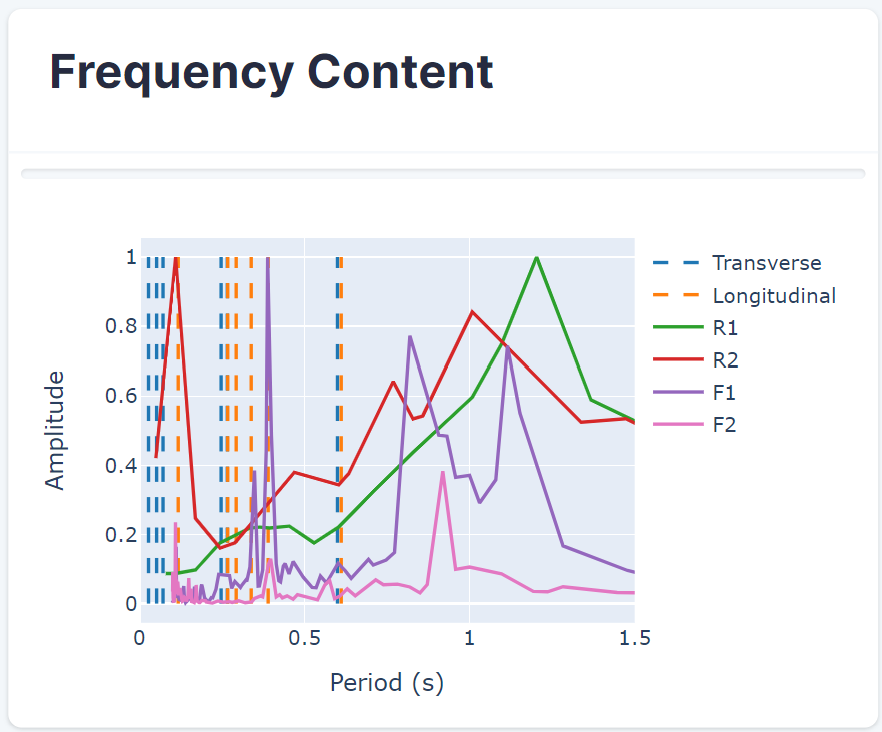
\includegraphics[width=.7\linewidth]{Part II/figures/predictors/freq_content2.png}
\caption{Example system identification prediction frequency content plot.}
\label{fig:sysid_example_freq_content}
\end{figure}
\begin{figure}[h!]
\centering
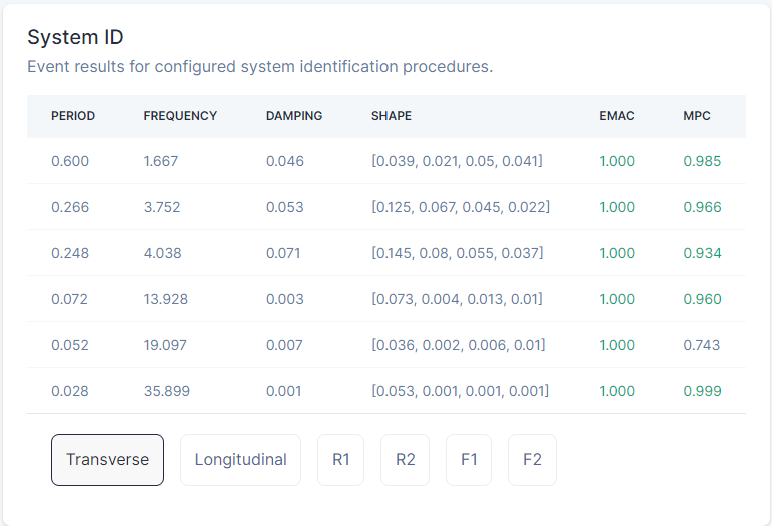
\includegraphics[width=.7\linewidth]{Part II/figures/predictors/sysid_example_results2.png}
\caption{Example system identification prediction results table.}
\label{fig:sysid_example_results}
\end{figure}
